\documentclass[a4paper,11pt,oneside]{article}
\usepackage{amsmath}
\usepackage{graphicx}
\author{Bhavishya Mittal}
\title{Assignment7}
\begin{document}
%\pagestyle{headings}
\maketitle
\newpage

\section*{School Algorithm}
Long multiplication is the method of multiplication that is commonly taught to elementary school students 
throughout the world. It can be used on two numbers of arbitrarily large size or number of decimal digits. 
The numbers to be multiplied are placed vertically over one another with their least significant digits aligned. 
The top number is named the multiplicand and the lower number is the multiplier. The result of the 
multiplication is the product.\\

For example, we can multiply 198 * 42. 
The number with more digits is usually selected as the multiplicand: 
This will be done as:\\

\begin{figure}[!h]
\rotatebox{-90}{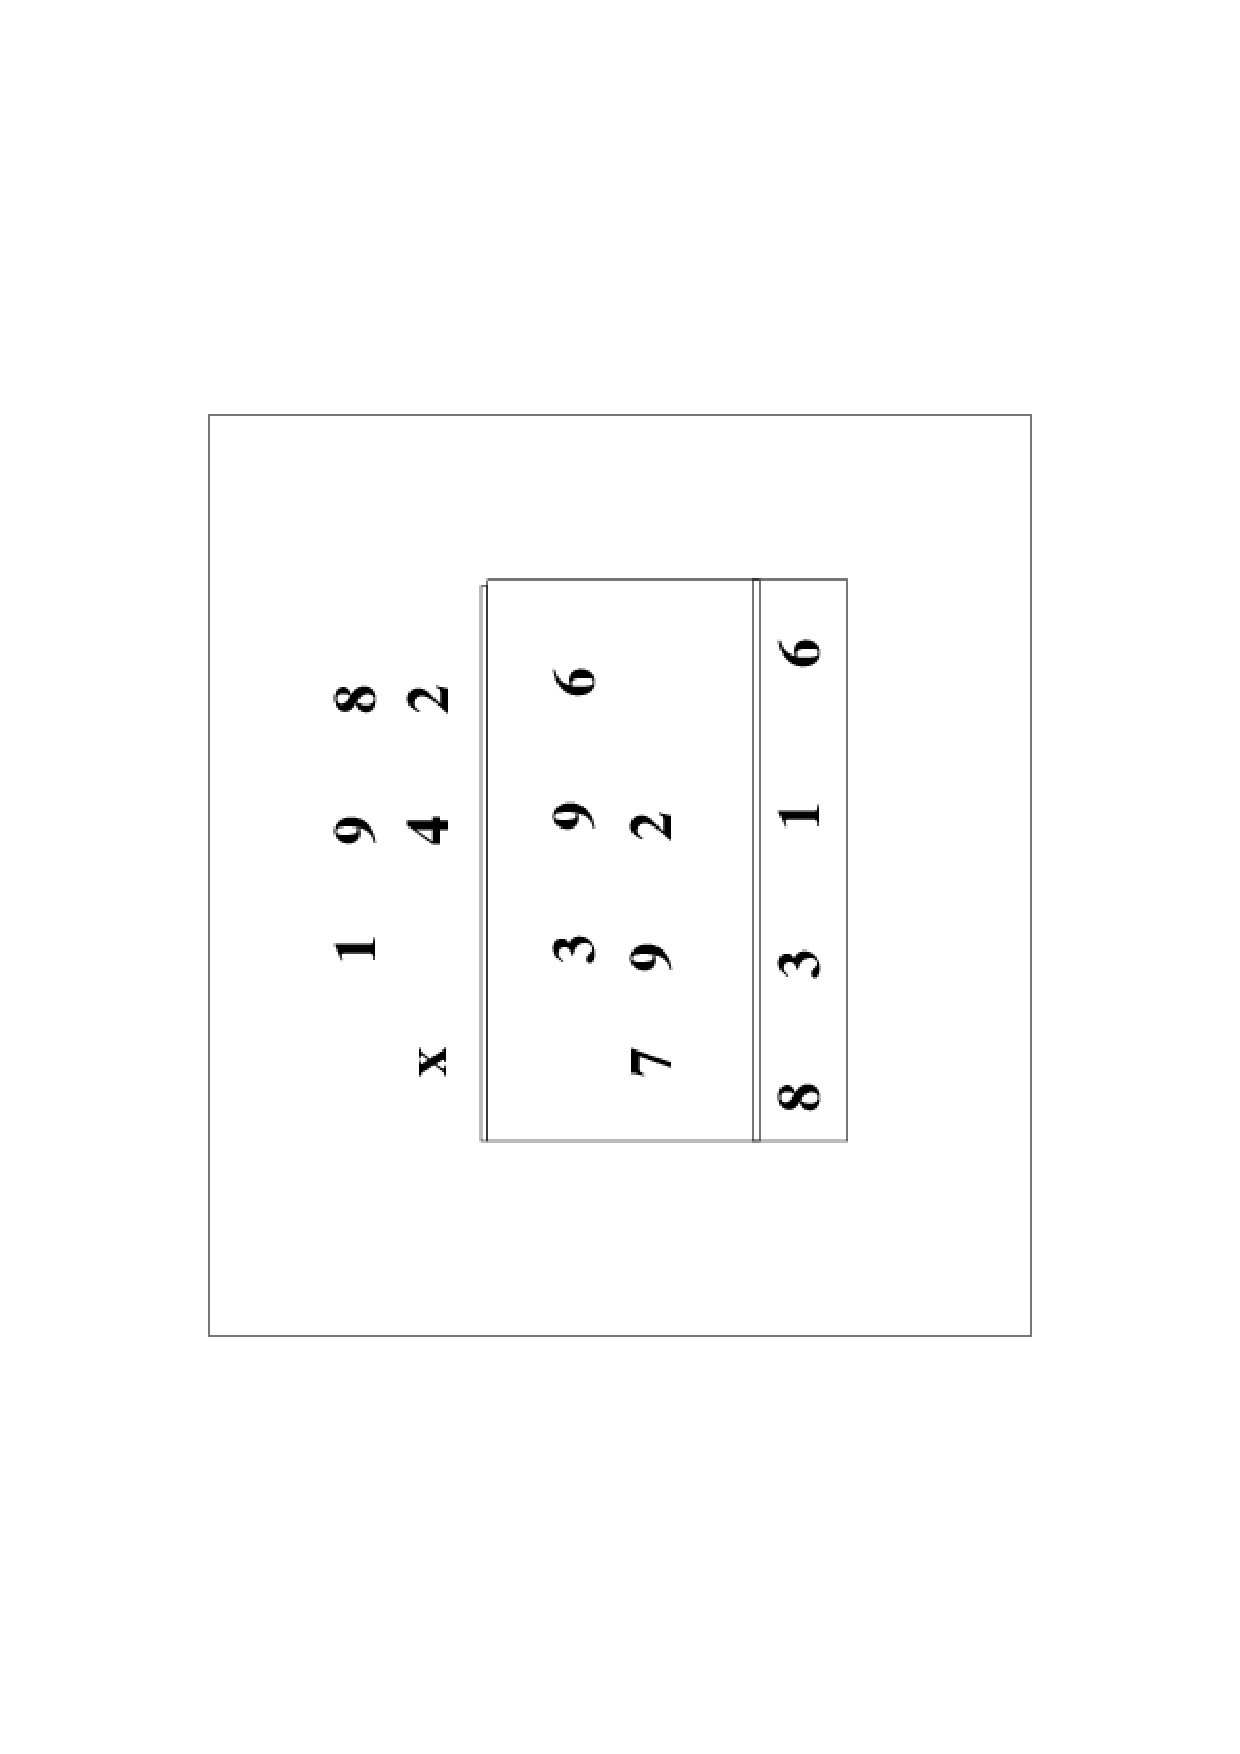
\includegraphics[scale=0.4]{pic}}
\caption{example to explain algorithm}
\end{figure}

\begin{figure}[!h]
\centerline{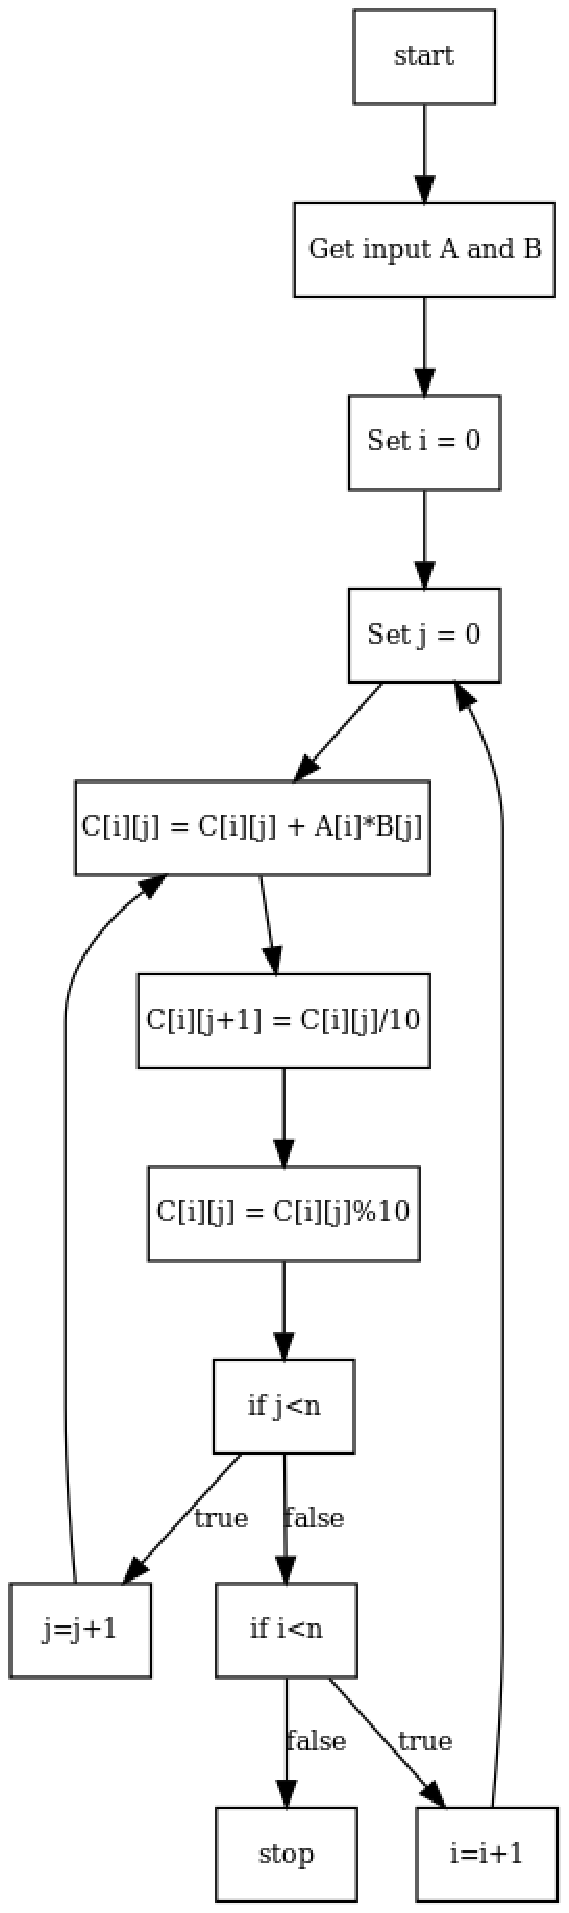
\includegraphics[scale=0.4]{flowchart}}
\caption{flowchart}
\end{figure}
The long multiplication algorithm starts with multiplying the multiplicand by the least 
significant digit of the multiplier to produce a partial product, then continuing this 
process for all higher order digits in the multiplier. Each partial product is right-aligned 
with the corresponding digit in the multiplier.
 
\section*{Characteristics}
\textbf{Pseudo-code:}\\
\hspace{10mm}
for($i$=0 to n-1) \\
\hspace{20 mm}
for($j$=0 to n-1) \\
\hspace{20 mm} \{\\
\hspace{30 mm}
$C$[$i$][$j$]+=$A$[$i$]*$B$[$j$] \\
\hspace{30 mm}
$C$[$i$][$j+1$]+=$C$[$i$][$j$]/10 \\
\hspace{30 mm}
$C$[$i$][$j$]=$C$[$i$][$j$]\%10 \\
\hspace{20 mm} \}\\
\flushleft
\textbf{Time Complexity:} \\
 The inner loop runs in $O(n)$ time and the outer loop ensures that the inner loops runs $n$ times. Thus the complexity of
 the above algorithm is $O(n*n)$ i.e. $O(n^2)$.
\end{document}
